% CVS info
\RCS$Revision: 1.0 $
\RCS$Date: 2008/04/13 04:21:28 $
%%%%%%%%%%%%% ptdr definitions %%%%%%%%%%%%%%%%%%%%%

%------------------------------------------------------------------------------
%%% put your own definitions here:
 
%%%%%%%%%%%%%%%%
% Declarations %
%%%%%%%%%%%%%%%%
%\def\bb{$\mathrm{b}\overline{\mathrm{b}}\;$}
%\def\cc{$\mathrm{c}\overline{\mathrm{c}}\;$}
\def\bb{$b\overline{b}\;$}
\def\cc{$c\overline{c}\;$}
\def\ttbar{$t\overline{t}\;$}
\def\mttbar{$m_{t\overline{t}}\;$}
\def\Zp{${Z'}\;$}
\def\ddZ{$\mathrm{d}\overline{\mathrm{d}}$}
\def\ss{$\mathrm{s}\overline{\mathrm{s}}\;$}
%\def\ttbar{$\mathrm{t}\overline{\mathrm{t}}\;$}
\def\ssZ{$\mathrm{s}\overline{\mathrm{s}}$}
\def\zqq{$\mathrm{Z} \rightarrow \mathrm{q}\overline{\mathrm{q}}\;$}
\def\zcc{$\mathrm{Z} \rightarrow \mathrm{c}\overline{\mathrm{c}}\;$}
\def\zbb{$\mathrm{Z} \rightarrow \mathrm{b}\overline{\mathrm{b}}\;$}
\def\zuuZ{$\mathrm{Z} \rightarrow \mathrm{u}\overline{\mathrm{u}}$}
%\def\gev{~GeV/$c\;$}
\def\gevc{~GeV/$c\;$}
\def\gevcc{~GeV/$c^{2}\;$}
\def\mum{~$\mu$m$\;$}
\def\pt{$p_T\;$}
\def\ptZ{$p_T$}
\def\Et{$E_T\;$}
\def\EtZ{$E_T$}
\def\ip{$IP\;$}
\def\ipZ{$IP$}
\def\dca{$dca\;$}
\def\prob{${\cal P}_{jet}\;$}
\def\probZ{${\cal P}_{jet}$}
\def\dr{$\Delta R\;$}
\def\pscat{$p_{scat}\;$}
\def\pscatZ{$p_{scat}$}
\def\sip{${\cal S}_{IP}\;$}
%\def\ptrel{$p_T^{\rm rel}}
\def\ptrel{$p_{Trel}\;$}
%\def\ptrelZ{$p_{Trel}$}
\def\tag{${\cal P}_{jet}^+<$}
%%%%%%%%%%%%%%%  Title page %%%%%%%%%%%%%%%%%%%%%%%%
% select one of the following and type in the proper number:
\cmsNoteHeader{2008/0XX}

\title{\bf An Update to the System8 Method to
        Measure the $b$ tagging Performance using a Muon in Jets Sample}

\author[purdue]{Pratima Jindal}
\author[fnal]{Francisco Yumiceva}
\address[fnal]{Fermi National Accelerator Laboratory, Batavia, Illinois USA}  
\address[purdue]{Purdue University Calumet, Hammond, Indiana, USA}
\date{\today}
  
\abstract{
This note describes 
}

% these need to be filled in by hand
\hypersetup{%
pdfauthor={Francisco Yumiceva},%
pdftitle={CMS Note 2008/0XX},%
pdfsubject={CMS},%
pdfkeywords={CMS, physics, btagging, muon,b}}


\maketitle %maketitle comes after all the front information has been supplied

%%%%%%%%%%%%%%%%%%%%%%%%%%%%%%%%  Begin text %%%%%%%%%%%%%%%%%%%%%%%%%%%%%
 
%DB
\setcounter{page}{2}
%DB
 
\section{Introduction}

New phenomena are expected to be discovered at the LHC. The
top sector could be the regime where we observe new physics in
 14 TeV collisions. For example, new 
resonances could appear which decay to \ttbar pairs.

\label{sec:intro}

\section{Selection Criteria and Simulation Datasets}
\label{sec:samples}

This study is based on three different Monte Carlo samples denoted QCD, 
inclusive $t\bar{t}+0$jets and $pp\rightarrow \mu +X$. The QCD sample 
was generated in different $\hat{p}_T $ bins at generator level. All
samples were generated with PYTHIA~\cite{ref:pythia}, except for the $t\bar{t} $ sample 
that was generated with ALPGEN~\cite{ref:alpgen}. All samples were simulated with 
CMSSW\_1\_4\_X and reconstructed with CMSSW\_1\_5\_2 as part of the CSA07
production. The $pp\rightarrow \mu +X $ sample is QCD minbias events with
muon $p_T > 3$~GeV/c. The muon is selected at the generator level. This
sample does not include muons produced by pion or kaon decays or by
punch-through. Thus, the light flavor jet contribution is much
lower than in the inclusive QCD sample.

The analysis is based on samples that have at least two reconstructed jets 
and a non-isolated muon close to one of the jets. The jets are reconstructed 
using the ITERATIVECONE5 algorithm~\cite{ref:iterativecone5} and corrected by a generator to 
reconstruction calibration factor. The jets and the muons in the event are
selected using the criteria described in the CMS Analysis 
Note~\cite{ref:btag_oldnote}.

Two samples are used in the analysis, defined as follows:
\begin{itemize} 
\item The  muon-in-jet+away-jet sample contains two reconstructed jets
and a non-isolated muon with $\Delta R(\mu,{\rm jet})<0.4$. In case 
more than one muon is found within a cone of $\Delta R<0.4$ of the jet, the 
muon with the highest $p_T$ is taken. For this study, the jet containing the 
muon will be denoted ``muon-jet",  and the other jet will be denoted the 
``away-jet''. If in a given event both jets contain muons, both will be 
counted as muon-jet. 
\item The muon-in-jet+tagged-away-jet sample is a subset of the 
muon-in-jet+away-jet sample, where the away-jet is tagged as a $b$ jet. 
\end{itemize}

Table~\ref{tab:samples} summarizes the samples used, and the number 
of events available.
For muon-jets the \ptrel is defined as the transverse momentum of the muon 
relative to the direction of the total muon-jet momentum vector,
 
\begin{equation}
p_{Trel}=\frac{|\vec{p^{\mu}} \times \vec{p^{\mu + {\rm jet}}}|}{|p^{\mu + {\rm jet}}|}.
\end{equation}

\begin{table}[bth]
 \begin{center}
 \begin{tabular}{l|r|r|r}
Sample                 & Events  & muon-in-jet & muon-in-jet+away-jet \\ \hline
QCD $\hat{p_T}$ 15-20  & 1286976 &    398      &       15 \\
QCD $\hat{p_T}$ 20-30  & 750966  &   864       &      59 \\
QCD $\hat{p_T}$ 30-50  & 1160479 &   5334      &      649 \\
QCD $\hat{p_T}$ 50-80  & 900240  & 11428       &    2390 \\
QCD $\hat{p_T}$ 80-120  & 1248757 &  27858     &      8592 \\
QCD $\hat{p_T}$ 120-170  & 1260951&   41667    &      16946 \\
QCD $\hat{p_T}$ 170-230  & 837547 &  36071     &     17714 \\
QCD $\hat{p_T}$ 230-300  & 760840 &  40190     &     22891 \\
QCD $\hat{p_T}$ 300-380  & 1225037&   73804    &      46954 \\
QCD $\hat{p_T}$ 380-470  & 1196202&   80258    &      55228 \\
QCD $\hat{p_T}$ 470-600  & 1226113&   90975    &      66464 \\
QCD $\hat{p_T}$ 600-800  & 546080 &  44122     &     33859 \\
QCD $\hat{p_T}$ 800-1000  & 717958  &   63664  &        50699 \\ \hline
inclusive $t\bar{t}+0$jets& 1511164 &    339947 &       259662 \\ \hline
$pp\rightarrow \mu +X$    & 18664210 &    611771 &      71519 \\ \hline

 \end{tabular}
 \end{center}
\caption[]{Summary of the total number of events from the CSA07 MC samples.}
\label{tab:samples}
\end{table}


%\label{sec:samples}
\clearpage
\section{Efficiency of the soft muon tagger}

In this section we use the System8 method to measure the efficiency of a 
simple Soft Muon Tagger (SLT) given by a cut on the \ptrel distribution of the 
muon. To ensure that the two taggers are independent and the correlation 
coefficients are close to unity, we modified the Track Counting tagger.
In the Track Counting tagger for each selected track in a jet, the impact 
parameter significance is computed. The jet is tagged by the Track Counting 
algorithm if the number of tracks with an impact parameter significance 
exceeding a given cut is greater than a discriminator value.

To create a life time tagger not involving the muon track we modified 
the jet track associator. The Jet track associator  loops over all the jets 
in an event and associates the tracks to a jet if they lie within a cone of 
0.5. We modify the Jet track associator to look for the good muons using the
criteria.
\begin{itemize} 
\item   number of Hits in the track $ \ge $ 8;
\item   $\mu $ Pt $ \ge $ 6;
\item   normalized $\chi^{2} \le 5$,
\end{itemize}   
and reject the good muon tracks from the track collection and associate rest 
of the tracks to jets. The modified jets with no muon tracks are then used 
for Track Counting method giving a modified Track counting b-tagging algorithm.

Figure~\ref{fig:Performanceplot} shows the performance plots
 comparing the modified Track Counting tagger with the Track Counting tagger
for the QCD RECO sample in the \pt range 80 to 120 GeV. Even though the 
performance of the Modified Track Counting is somewhat worse, its seperation
power is still sufficient to enrich the sample in b-jets and allow us to use 
System8 to measure the efficiency of the SLT algorithm.


\begin{figure}[htbp]
  \begin{center}
    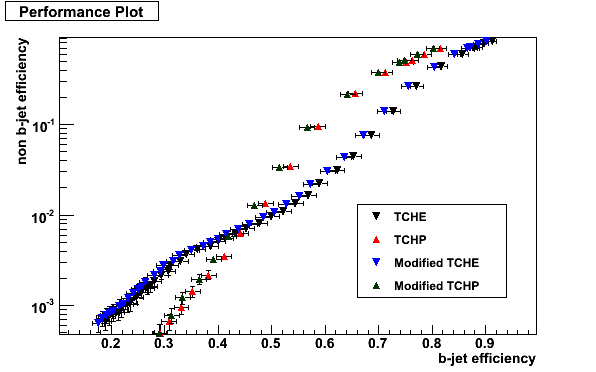
\includegraphics[width=90mm]{Figures/QCD_80_120.png}
  \end{center}
  \caption{Performance Plot comparing the performance of the default and 
modified Track Counting Algorithm for QCD 80-120 GeV sample.}
  \label{fig:Performanceplot}
\end{figure}


The Modified Track Counting tagger has been used as one of the taggers of
System8 to determine the efficiency for the Soft Muon Tagger





\clearpage

%\section{Summary and Conclusions}


 The System8 method has been extended to consider correlations for the soft
muon tagger. We now have a better convergence range in jet $p_T$ for System8
method as compared to the previous analysis~\cite{ref:btag_oldnote}. Along with
the b-tagging efficiency we also studdied the charm+light jet tagging 
efficiency using the System8 method. The method was applied to the 
$pp\rightarrow \mu +X$, $t\bar{t}+0$~jets and QCD samples for the three 
operating points of the Track Counting and the Track Probability tagger and the
pTrel(soft muon tagger) . The average solutions from System8 are in good 
agreement with the expected efficiencies obtained from the MC truth information.
The b-tag efficiency has been measured as a function of jet $p_T$ using a coarse
binning in $p_T$ for the $pp\rightarrow \mu +X$ sample. The agreement between 
the measured and expected b-tag efficiency from MC truth is good for the Track 
Counting and pTrel taggers, but the agreement is not very good for the 
Jet Probability tagger for the loose and medium operating points.

 We would like to incorporate some improvements/revisions into the Performance 
measurement package like cross-checking that we use the muon with the highest 
$p_T$ to calculate the pTrel, improving the muon identification, 
using a muon trigger, and try to get rid of the tiny contamination from other 
processes with a muon-in-jet like the $J/\Psi $ and charm quark decay.

%\label{sec:conclusions}

\section{Acknowledgment} 
We would like to thank ...

\appendix
%DB \input{Correlations}
%DB \label{sec:correlations}

\begin{thebibliography}{99}

\bibitem{ref:pythia}
T.~Sj{\"o}strand, L.~Lonnblad and S.~Mrenna, hep-ph/0108264 (2001).

\bibitem{ref:root}
ROOT analysis system 
http://root.cern.ch/

\end{thebibliography}
 
 
%%%%%%%%%%%%%%%%%%%%%%%%%%%%%%%%%%%%%%%%%%%%%%%%%%%%%%%%%%%%%%%%%%%%%%%%%%%%%%%

%%%%%%%%%%%%%%%%%%%%%%%%%%%%%%%%%%%%%%%%%%%%%%%%%%%%%%%%%%%%%%%%%%%%%%%%%%%%%%%
\end{document}
